\subsection{Moduły}

Klasy w programie C\#-owym pogrupowane są w rozłącznych przestrzeniach nazw ({\em namespace'ach}). 
Dostęp do klas umieszczonych w określonej przestrzeni nazw możliwy jest dzięki konstrukcji

\begin{scriptsize}
\begin{verbatim}
NazwaPrzestrzeniKlas.NazwaFunkcji
\end{verbatim}
\end{scriptsize}

na przykład

\begin{scriptsize}
\begin{verbatim}
System.Console.WriteLine(...);
\end{verbatim}
\end{scriptsize}

bądź zadeklarowaniu na początku programu chęci dostępu do określonej przestrzeni nazw

\begin{scriptsize}
\begin{verbatim}
using NazwaPrzestrzeniKlas
\end{verbatim}
\end{scriptsize}

dzięki czemu do funkcji z tej przestrzeni nazw można odwoływać się bez poprzedzania
ich nazw nazwą przestrzeni nazw. Podział programu na różne przestrzenie nazw zwykle wynika
z logicznego podziału programu na moduły. Nie wnikając w strukturę modułu, powiedzmy tylko że zawiera on
opis klas, przy czym moduł wykonywalny (*.exe) różni się od modułu-biblioteki (*.dll) tylko tym, że 
w jednej z klas zawiera kod startowy (tu: funkcję Main()). 

Przykład najprostszego modułu:

\begin{scriptsize}
\begin{verbatim}
/* Wiktor Zychla, 2003 */
using System;

namespace ExampleModule
{ 
  public class ExampleClass
  {    
    public int Metoda()
    {
      return 17;
    }
  }
}

C:\Example>csc.exe /target:library exampleM.cs
Microsoft (R) Visual C# .NET Compiler version 7.00.9466
for Microsoft (R) .NET Framework version 1.0.3705
Copyright (C) Microsoft Corporation 2001. All rights reserved.
\end{verbatim}
\end{scriptsize}

Przykład programu korzystającego z modułu:

\begin{scriptsize}
\begin{verbatim}
/* Wiktor Zychla, 2003 */
using System;
using ExampleModule;

namespace Example
{ 
  public class CMain
  {    
    public static void Main()
    {
      ExampleClass e = new ExampleClass();
      Console.WriteLine( e.Metoda() );
    }
  }
}

C:\Example>csc.exe /reference:exampleM.dll example.cs
Microsoft (R) Visual C# .NET Compiler version 7.00.9466
for Microsoft (R) .NET Framework version 1.0.3705
Copyright (C) Microsoft Corporation 2001. All rights reserved.
\end{verbatim}
\end{scriptsize}

Od tej pory moduł główny i biblioteka mogą być kompilowane niezależnie, zaś prawidłowe wykonanie kodu
modułu możliwe będzie tylko wtedy, kiedy biblioteka będzie dostępna dla środowiska uruchomieniowego
w czasie wykonania programu, czyli na przykład znajdzie się w tym samym folderze co moduł główny.

\subsection{Refleksje}

Możliwość odczytywania i analizy metadanych, czyli opisu typów z już istniejącego kodu nosi 
nazwę {\em refleksji}. Refleksje są jednym z najpotężniejszych mechanizmów platformy .NET.

Przede wszystkim każdy typ w systemie może być zidentyfikowany, ponadto można utworzyć zmienną 
typową podając nazwę typu.

\begin{scriptsize}
\begin{verbatim}
/* Wiktor Zychla, 2003 */
using System;

namespace Example
{
  public class CExample
  {
    static void PrintTypeInfo( Type t )
    {
      Console.WriteLine( "Definicja {0} znajduje się w module {1}.", 
                           t, t.Module );
    }

    public static void Main(string[] args)
    {
      string s = String.Empty;
      PrintTypeInfo( s.GetType() );

      Type t = Type.GetType( "Example.CExample" );
      PrintTypeInfo( t ); 
    }
  }
}

C:\Example>example.exe
Definicja System.String znajduje się w module CommonLanguageRuntimeLibrary.
Definicja Example.CExample znajduje się w module example.exe.
\end{verbatim}
\end{scriptsize}

Każdy moduł może być przeanalizowany pod kątem zawartych w nim typów:

\begin{scriptsize}
\begin{verbatim}
/* Wiktor Zychla, 2003 */
using System;
using System.Reflection;

namespace Example
{	  
  class CExample
  {  	
    static Assembly GetAssembly(string[] args)
    {
      Assembly assembly;
      if (0 == args.Length)
      {
          assembly = Assembly.GetExecutingAssembly();
      }
      else
      {
          assembly = Assembly.LoadFrom(args[0]);
      }
      return assembly;
    }

    public static void Main(string[] args)
    {
      Assembly assembly = GetAssembly(args);
      if (null != assembly)
      {
        Console.WriteLine("Informacje o typach dla {0}", assembly);

        Type[] types = assembly.GetTypes();
        foreach(Type type in types)
        {
          Console.WriteLine("\nTyp: {0}", type);
          foreach(MemberInfo member in type.GetMembers())
          {
            Console.WriteLine("\tSkladowa: {0}", member);
          }
        }
      }      
    }
  }
}

C:\Example>example.exe
Informacje o typach dla Example, Version=1.0.1176.39934, Culture=neutral, Public
KeyToken=null

Typ: Example.CExample
        Skladowa: Int32 GetHashCode()
        Skladowa: Boolean Equals(System.Object)
        Skladowa: System.String ToString()
        Skladowa: Void Main(System.String[])
        Skladowa: System.Type GetType()
        Skladowa: Void .ctor()
\end{verbatim}
\end{scriptsize}

Za pomocą tego programu można obejrzeć listy typów w modułach .NET, na przykład System.Windows.Forms.dll
czy MSCORLIB.DLL.

Mechanizm refleksji może być wykorzystany do dynamicznego tworzenia instancji obiektów, 
gdy znany jest typ obiektu. Można w taki sposób zrealizować dynamiczne łączenie
modułów - łączenie nie w czasie kompilacji, tylko w czasie wykonania.

\begin{scriptsize}
\begin{verbatim}
/* Wiktor Zychla, 2003 */
using System;
using System.Reflection;

namespace Example
{
  public class CTest
  {
    public int testVal;

    public CTest() {}

    override public string ToString()
    {
      return "CTest: " + testVal.ToString();
    }
  }

  public class CExample
  {
    public static void DynamicObjectCreation( Type t )
    {
      int i;
      object o;

      ConstructorInfo   c;
      FieldInfo         f;

      ConstructorInfo[] ci;
      ParameterInfo[]   pi;
      FieldInfo[]       fi;	
				
      ci = t.GetConstructors();
      for (i=0; i<ci.Length; i++)
      {
        c = ci[i];

        pi = c.GetParameters();
        if ( pi.Length == 0 )
        {
          o = c.Invoke(null);

          fi = t.GetFields();					
          for ( int j=0; j<fi.Length; j++ )
          {
            f = fi[j];
            if ( f.FieldType == Type.GetType("System.Int32" ) )
               f.SetValue( o, 17 );
          }

        Console.WriteLine( "Typ {0}, ToString(): {1}", o.GetType(), o );
      }
    }
 
    public static void Main()
    {
      DynamicObjectCreation( Type.GetType( "Example.CTest" ) );
    }
  }
}

C:\Example>example.exe
Typ Example.CTest, ToString() CTest: 17
\end{verbatim}
\end{scriptsize}

\subsection{Atrybuty}

Myśląc o typach i obiektach, które są instancjami odpowiednich typów, wyraźnie rozróżniamy te dwa światy.
W chwili wykonania programu  instancje obiektów są elementami dynamicznymi - pojawiają się i giną 
zależnie od woli programisty. Tworząc, modyfikując i niszcząc obiekty programista pracuje na 
{\em poziomie języka}, czyli na poziomie konkretnych wartości wypełniających szablony jakimi są typy.
Dzięki mechanizmowi refleksji, programista w trakcie działania programu może również pracować na
{\em poziomie metajęzyka}, czyli na poziomie informacji o typach: o ich składowych, o zależnościach między typami.

Mechanizm atrybutów to kolejny mechanizm z poziomu metajęzyka. Atrybuty pozwalają rozszerzyć 
definicje typów o dodatkowe informacje, możliwe do wydobycia dzięki refleksjom. Wyobraźmy sobie pewien 
abstrakcyjny scenariusz, w którym każdy typ pojawiający się w programie byłby określony 
jako niebieski, czarny lub zielony. 
Uwaga - nie {\em instancja typu} (czyli konkretna zmienna), ale właśnie typ sam
w sobie. Taka informacja mogłaby być na przykład jakąś dodatkową wskazówką dla kompilatora lub być w jakiś
inny sposób wykorzystana w trakcje działania aplikacji. 

Scenariusz ten zrealizujemy właśnie dzięki atrybutom. Atrybuty są klasami dziedziczącymi z klasy
{\bf Attribute}, których instancje dzięki specjalnej składni można związać z klasami bądź ich składowymi.

\begin{scriptsize}
\begin{verbatim}
/* Wiktor Zychla, 2003 */
using System;

namespace Example
{
  public class KolorKlasyAttribute : Attribute
  {
    public KolorKlasyAttribute( string kolor )
    {
      this.kolor = kolor;
    }
    public string Kolor
    {
      get { return kolor; }
    }

    string kolor;
  }

  [KolorKlasy( "zielony" )]
  public class Typ1
  {
  }

  [KolorKlasy( "niebieski" )]
  public class Typ2
  {
  }

  public class CMainForm 
  {   
    public static void Main()
    {
      Type type;

      // zbadaj Typ1
      type = typeof( Typ1 );
      foreach ( Attribute a in type.GetCustomAttributes( true ) )
      {
        KolorKlasyAttribute kolorKlasy = a as KolorKlasyAttribute;
        if ( kolorKlasy != null )
          Console.WriteLine( "Typ {0} ma kolor {1}", type.Name, kolorKlasy.Kolor ); 
      }       

      // zbadaj Typ2
      type = typeof( Typ2 );
      foreach ( Attribute a in type.GetCustomAttributes( true ) )
      {
        KolorKlasyAttribute kolorKlasy = a as KolorKlasyAttribute;
        if ( kolorKlasy != null )
          Console.WriteLine( "Typ {0} ma kolor {1}", type.Name, kolorKlasy.Kolor ); 
      }       
    }
  }
}

C:\Example>example.exe
Typ Typ1 ma kolor zielony
Typ Typ2 ma kolor niebieski
\end{verbatim}
\end{scriptsize}

\subsubsection{Predefiniowane atrybuty}

W świecie .NET istnieje kilkanaście gotowych atrybutów, których można użyć do poinformowania
kompilatora o specjalnych właściwościach typów lub ich składowych. W kolejnych rozdziałach zobaczymy 
przykłady użycia atrybutu {\bf [Serializable]}, który służy do poinformowania kompilatora o tym, że
klasa może być serializowana. Zobaczymy także przykłady użycia atrybutów {\bf [DllImport]} i
{\bf [StructLayout]}, które umożliwiają zdefiniowanie funkcji i struktur odwołujących się
do funkcji i struktur ze zwykłych, niezarządzanych bibliotek Windowsowych.

Tu wspomnimy jedynie o atrybutach, pozwalających na określenie informacji o pliku, będącym efektem kompilacji.
Można je umieścić w dowolnym miejscu w kodzie, bowiem odnoszą się do całego modułu, będącego wynikiem
kompilacji. Efekt ich dodania można obejrzeć na zakładce {\bf Wersja}, w oknie właściwości pliku.

\begin{scriptsize}
\begin{verbatim}
[assembly: AssemblyTitle("Moja Aplikacja numer 1")]
[assembly: AssemblyDescription("Opis mojej aplikacji")]
[assembly: AssemblyCompany("Moja firma")]
[assembly: AssemblyProduct("A1")]
[assembly: AssemblyCopyright("Moja firma")]
[assembly: AssemblyVersion("1.7.1.0")
\end{verbatim}
\end{scriptsize}

\subsection{Kod niebezpieczny}

Programiści, którzy dobrze znają C czy C++, czasami bywają w pierwszym kontakcie rozczarowani brakiem
bezpośredniej kontroli nad zarządzaniem pamięcią oraz brakiem wskaźników w C\#.

Brak możliwości sterowania destrukcją obiektów jest w pełni uzasadniony. Z pewnością w pewnych przypadkach
możliwe jest napisanie przez programistę kodu, który samodzielnie zarządza przydzielaniem i zwalnianiem pamięci,
jednak w większości przypadków automat i tak robi to lepiej. Jeśli komuś bardzo zależy na możliwości
pełnej kontroli nad przydzielaniem i zwalnianiem pamięci - niech po prostu programuje w C.

Co zaś do wskaźników, to okazuje się, że istnieje w C\# możliwość korzystania z nich. Po prostu fragment kodu
korzystający ze wskaźników musi być oznakowany kwalifikatorem {\em unsafe}. Choć nazwa sugeruje, że kod
taki jest w jakiś sposób niebezpieczny, tak naprawdę chodzi tu tylko o obejście dość restrykcyjnego
systemu typów C\#, który w żaden sposób nie potrafiłby przepuścić kodu upstrzonego wskaźnikami. Oprócz kodu
{\em niebezpiecznego} możliwy jest również kod {\em niezarządzany}. Z kodem niezarządzanym mamy do czynienia
przy uruchamianiu z kodu C\#-owego modułów COM lub COM+, napisanych w Visual Basicu lub C++. Kod
niezarządzany sam zajmuje się obsługą pamięci i nie korzysta z bibliotek platformy \NET{}.

Kod niebezpieczny musi być kompilowany z przełącznikiem {\em /unsafe}.

\begin{scriptsize}
\begin{verbatim}
/* Wiktor Zychla, 2003 */
using System;

namespace Example
{
  public class CExample
  {
    unsafe public static void Swap(int* pi, int* pj)
    {
        int tmp = *pi;
        *pi = *pj;
        *pj = tmp;
    }

    public static void Main(string[] args)
    {
        int i = 17;
        int j = 23;

        Console.WriteLine("Przed zamianą: i = {0}, j = {1}", i, j);
        unsafe { Swap(&i, &j); }
        Console.WriteLine("Po zamianie:  i = {0}, j = {1}", i, j);
    }
  }
}
\end{verbatim}
\end{scriptsize}

W kodzie niebezpiecznym o wiele łatwiej popełnić niezamierzoną pomyłkę. Jednak złe odwołania 
do pamięci będą wyłapywane przez środowisko uruchomieniowe:

\begin{scriptsize}
\begin{verbatim}
/* Wiktor Zychla, 2003 */
using System;

namespace Example
{
  public class CExample
  {
    unsafe public static void Blad()
    {
        int  i;
        int* pi = &i;
        pi     += 10000;
        *pi     = 0;
    }

    public static void Main(string[] args)
    {
        unsafe { Blad(); }
    }
  }
}

C:\Example>example.exe

Unhandled Exception: System.NullReferenceException: Object reference not set to
an instance of an object.
   at Example.CExample.Blad()
   at Example.CExample.Main(String[] args)
\end{verbatim}
\end{scriptsize}

\subsection{Dokumentowanie kodu}
\label{dokumentowanieKodu}

Programiści bardzo niechętnie dokumentują kod, który tworzą. Z drugiej strony nawet kilka
słów komentarza bywa często bardzo cenne, zwłaszcza kiedy wraca się do kodu napisanego dawno temu.
Oczywiście istnieje możliwość tworzenia komentarzy w kodzie, jednak nie da się na podstawie takich
komentarzy zbudować niczego co mogłoby być jakąś formą dokumentacji całości kodu.

W C\# zaproponowano pewien jednolity sposób tworzenia komentarzy w kodzie jako tagów języka 
XML\footnote{Więcej o języku XML na stronie \pageref{section_XML}.}. Zobaczmy prosty przykład
komentarzy w kodzie programu, sposób tworzenia dokumentacji i ostateczną postać dokumentacji:

\begin{scriptsize}
\begin{verbatim}
/* Wiktor Zychla, 2003 */
using System;

namespace Example
{
    /// <summary>
    /// Klasa zawierająca kod startowy aplikacji.
    /// </summary>
    class CExample
    {
        /// <summary>
        /// Tutaj mógłby znaleźć się opis funkcji f.
        /// Opis ten może być dowolnie długi.
        /// </summary> 
        void f()
        {
        }
        /// <summary>
        /// Główna funkcja aplikacji.
        /// </summary>
        [STAThread]
        static void Main(string[] args) 
        {
        }

    }
}

C:\Example>csc.exe /doc:example.xml example.cs

<?xml version="1.0"?>
<doc>
    <assembly>
        <name>example</name>
    </assembly>
    <members>
        <member name="T:Example.CExample">
            <summary>
            Klasa zawierająca kod startowy aplikacji.
            </summary>
        </member>
        <member name="M:Example.CExample.f">
            <summary>
            Tutaj mógłby znaleźć się opis funkcji f.
            Opis ten może być dowolnie długi.
            </summary> 
        </member>
        <member name="M:Example.CExample.Main(System.String[])">
            <summary>
            Główna funkcja aplikacji.
            </summary>
        </member>
    </members>
</doc>
\end{verbatim}
\end{scriptsize}

\begin{figure}
\begin{center}
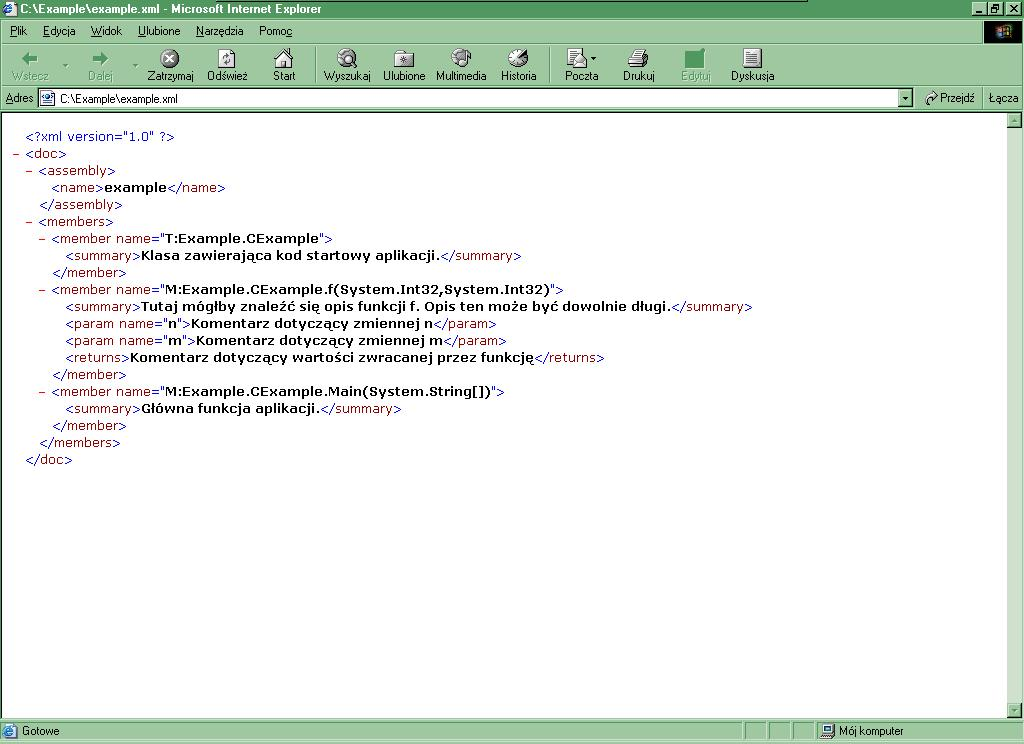
\includegraphics[width=0.75\textwidth]{./pic/w04}
\caption{Dokumentacja XML w przeglądarce Internetowej}
\end{center}
\end{figure}

Tworzenie dokumentacji w ten sposób jest szczególnie łatwe w Visual Studio .NET. Edytor kodu C\#
potrafi automatycznie zbudować odpowiedni szablon dokumentacji po wprowadzeniu przez programistę
znaku rozpoczęcia takiego komentarza, czyli ///. 
Istnieje kilkanaście różnych możliwych 
tagów XML jakimi można opatrywać różne elementy kodu, najbardziej przydaje się jednak możliwość pełnego
dokumentowania metod:

\begin{scriptsize}
\begin{verbatim}
/// <summary>
/// Tutaj mógłby znaleźć się opis funkcji f.
/// Opis ten może być dowolnie długi.
/// </summary> 
///<param name="n">Komentarz dotyczący zmiennej n</param>
///<param name="m">Komentarz dotyczący zmiennej m</param>
///<returns>Komentarz dotyczący wartości zwracanej przez funkcję</returns>
int f( int n, int m)
{
}
\end{verbatim}
\end{scriptsize}

Utworzony plik z dokumentacją może być otworzony na przykład przez przeglądarkę Internetową, jednak
można, za pomocą arkuszy stylów XSL, nadać mu własne formatowanie. Visual Studio .NET potrafi wykorzystać
tę możliwość do utworzenia elegancko sformatowanych stron HTML z dokumentacją.

\begin{figure}
\begin{center}
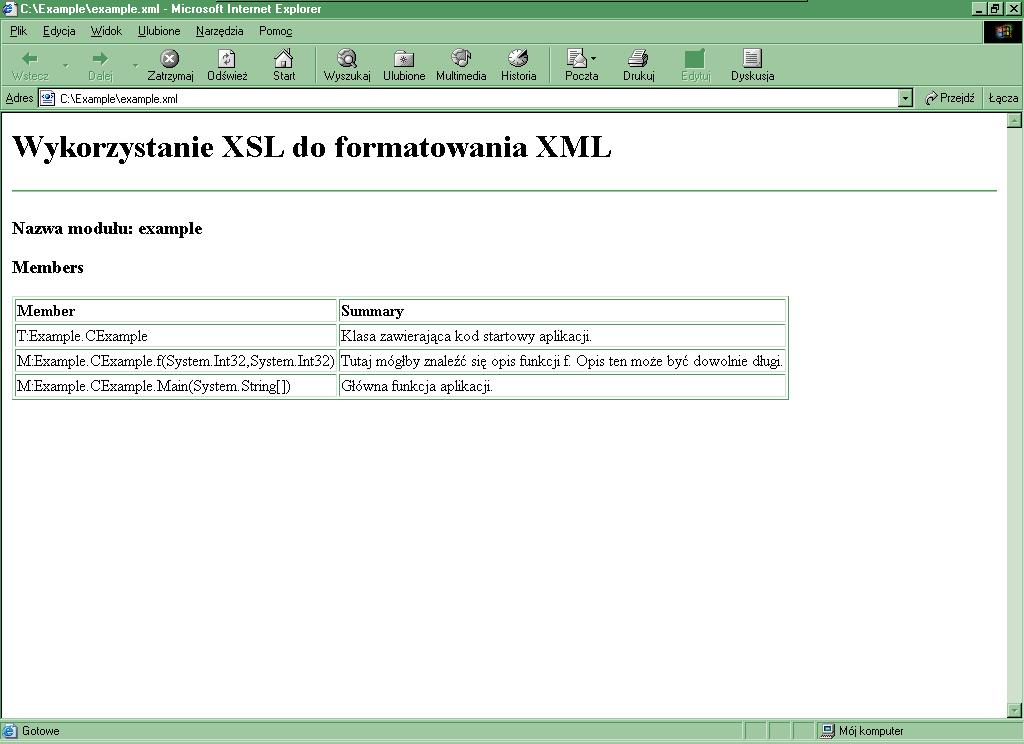
\includegraphics[width=0.75\textwidth]{./pic/w03}
\caption{Zastosowanie prostego arkusza stylów XSL, przedstawionego w tekście, do sformatowania dokumentacji XML}
\end{center}
\end{figure}

Wykorzystajmy dla przykładu bardzo prosty arkusz stylów:

\begin{scriptsize}
\begin{verbatim}
<xsl:stylesheet xmlns:xsl="http://www.w3.org/TR/WD-xsl">
<xsl:template match="/">
  <html><body>
    <h1>Wykorzystanie XSL do formatowania XML</h1>
    <hr/>
    <h3>
      Nazwa modułu: <xsl:value-of select="doc/assembly/name"/>
    </h3>
    <table border="1">
      <thead><h3>Members</h3></thead>
      <tbody>
        <tr>
          <td><b>Member</b></td>
          <td><b>Summary</b></td>
        </tr>
        <xsl:for-each select="doc/members/member">
          <tr>
            <td><xsl:value-of select="@name"/></td>
            <td><xsl:value-of select="summary/text()"/></td>
          </tr>
        </xsl:for-each>
      </tbody>
    </table>
  </body></html>
</xsl:template>
</xsl:stylesheet>
\end{verbatim}
\end{scriptsize}

i w pliku z dokumentacją XML dodajmy informację o arkuszu stylów:

\begin{scriptsize}
\begin{verbatim}
<?xml-stylesheet href="example.xsl" type="text/xsl"?> 
<?xml version="1.0"?>
<doc>
    <assembly>
        <name>example</name>
    </assembly>
    <members>
        <member name="T:Example.CExample">
            <summary>
            Klasa zawierająca kod startowy aplikacji.
            </summary>
        </member>
        <member name="M:Example.CExample.f(System.Int32,System.Int32)">
             <summary>
             Tutaj mógłby znaleźć się opis funkcji f.
             Opis ten może być dowolnie długi.
             </summary> 
            <param name="n">Komentarz dotyczący zmiennej n</param>
            <param name="m">Komentarz dotyczący zmiennej m</param>
            <returns>Komentarz dotyczący wartości zwracanej przez funkcję</returns>
        </member>
        <member name="M:Example.CExample.Main(System.String[])">
            <summary>
            Główna funkcja aplikacji.
            </summary>
        </member>
    </members>
</doc>
\end{verbatim}
\end{scriptsize}

\begin{figure}
\begin{center}
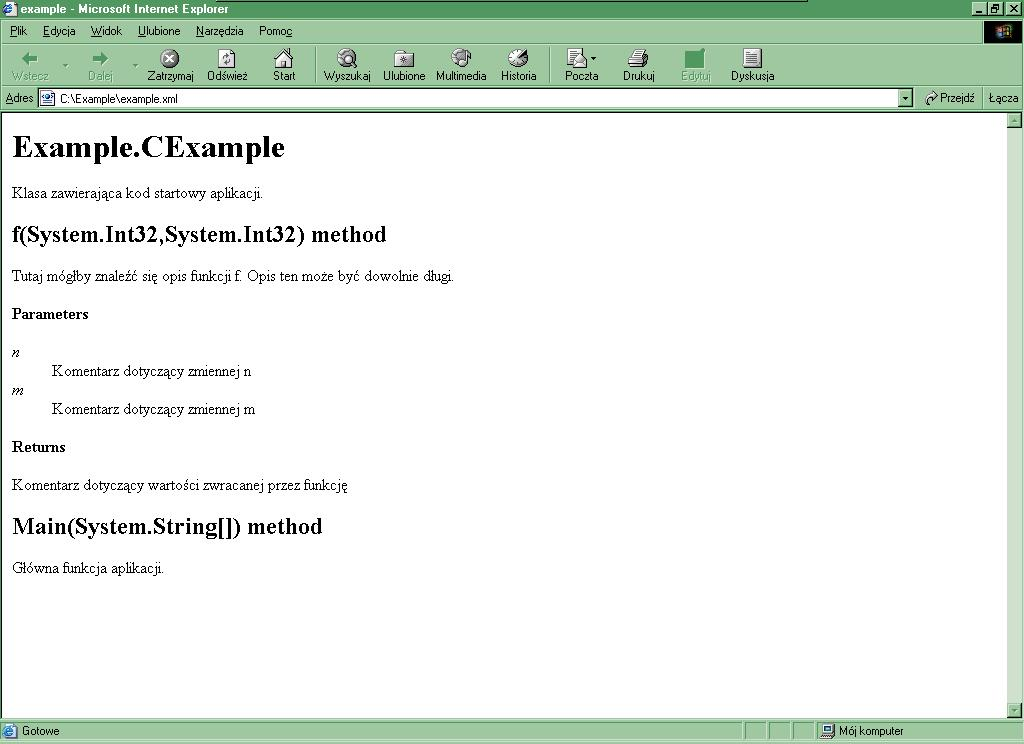
\includegraphics[width=0.75\textwidth]{./pic/w02}
\caption{Zastosowanie innego arkusza stylów XSL, programista ma tutaj całkowitą dowolność}
\end{center}
\end{figure}

\subsection{Dekompilacja kodu}
\label{csDekompilacja}

Rozważmy przykład prostego kodu:

\begin{scriptsize}
\begin{verbatim}
/* Wiktor Zychla, 2003 */
using System;

namespace NExample
{
  class CExample
  {
    public int i;
    public string s;

    public int Oblicz( int n )
    {
      int k = 0;
      for ( int l=0; l<n; l++ )
        k+=l;

      return k;
    }

    public CExample()
    {
      i = 0;
      s = String.Empty;
    }
  }

  class CMain
  {
    public static void Main()
    {
      CExample e = new CExample();
      Console.WriteLine( e.Oblicz(7).ToString() );
    }
  }
}
\end{verbatim}
\end{scriptsize}

\subsubsection{Dekompilacja do języka IL}

.NET Framework SDK zawiera m.in. dekompilator kodu, dzięki któremu można obejrzeć
kod IL-owy dowolnego modułu .NETowego\footnote{Dekompilator IL jest częścią .NET Framework SDK, 
kompilator IL jest częścią samego .NET Frameworka.}.
Dekompilator uruchamia się poleceniem {\em ildasm.exe}.

Dekompilator pozwala obejrzeć kod dowolnego obiektu w dowolnej klasie projektu. Oznacza to, że może być
nawet wykorzystany do podglądania kodu bibliotek .NET! 

Wykorzystajmy więc {\em Ildasm} do zdekompilowania metody {\em Main} z powyższego
przykładu:

\begin{scriptsize}
\begin{verbatim}
.method public hidebysig static void  Main() cil managed
{
  .entrypoint
  // Code size       27 (0x1b)
  .maxstack  2
  .locals init (class NExample.CExample V_0,
           int32 V_1)
  IL_0000:  newobj     instance void NExample.CExample::.ctor()
  IL_0005:  stloc.0    
  IL_0006:  ldloc.0
  IL_0007:  ldc.i4.7
  IL_0008:  callvirt   instance int32 NExample.CExample::Oblicz(int32)
  IL_000d:  stloc.1
  IL_000e:  ldloca.s   V_1
  IL_0010:  call       instance string [mscorlib]System.Int32::ToString()
  IL_0015:  call       void [mscorlib]System.Console::WriteLine(string)
  IL_001a:  ret
} // end of method CMain::Main
\end{verbatim}
\end{scriptsize}

oraz do zdekompilowania metody {\em CExample.Oblicz}:

\begin{scriptsize}
\begin{verbatim}
.method public hidebysig instance int32  Oblicz(int32 n) cil managed
{
  // Code size       24 (0x18)
  .maxstack  2
  .locals init (int32 V_0,
           int32 V_1,
           int32 V_2)
  IL_0000:  ldc.i4.0
  IL_0001:  stloc.0
  IL_0002:  ldc.i4.0
  IL_0003:  stloc.1
  IL_0004:  br.s       IL_000e
  IL_0006:  ldloc.0
  IL_0007:  ldloc.1
  IL_0008:  add
  IL_0009:  stloc.0
  IL_000a:  ldloc.1
  IL_000b:  ldc.i4.1
  IL_000c:  add
  IL_000d:  stloc.1
  IL_000e:  ldloc.1
  IL_000f:  ldarg.1
  IL_0010:  blt.s      IL_0006
  IL_0012:  ldloc.0
  IL_0013:  stloc.2
  IL_0014:  br.s       IL_0016
  IL_0016:  ldloc.2
  IL_0017:  ret
} // end of method CExample::Oblicz
\end{verbatim}
\end{scriptsize}

Struktura kodu pośredniego jest bardzo prosta, kompilator C\# nie stosuje praktycznie żadnych
optymalizacji. To reguła w świecie .NET - kompilator JIT podczas kompilacji kodu pośredniego do
kodu natywnego i tak dokonuje swoich optymalizacji, dlatego kompilatory języków nie muszą tego
robić na poziomie kompilacji kodu języka do kodu pośredniego.

Język IL będzie dokładniej omówiony w rozdziale \ref{langIL}

\begin{figure}
\begin{center}
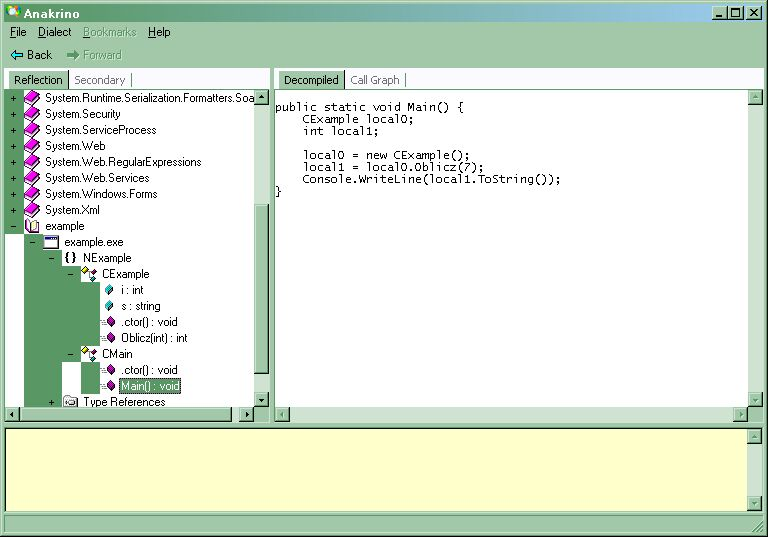
\includegraphics[width=0.75\textwidth]{./pic/w05}
\caption{Dekompilacja kodu IL do C\# w Anakrino}
\end{center}
\end{figure}

\subsubsection{Dekompilacja do C\#}

Czy można wyobrazić sobie narzędzie, które pozwalałoby odtwarzać kod C\# z binarium zawierającego kod pośredni?

Okazuje się, że tak. Najpopularniejszym w tej chwili dekompilatorem kodu C\# jest
{\bf Anakrino}. Zdekompilowany kod zawiera poprawne nazwy klas, metod i parametrów, niepoprawnie natomiast
odtwarzane są na przykład nazwy zmiennych lokalnych metod. Dzieje się tak, ponieważ nazwy zmiennych lokalnych
nie są przechowywane w kodzie pośrednim.

Zdekompilowana przez Anakrino kod metody {\em Main}:

\begin{scriptsize}
\begin{verbatim}
public static void Main() {
  CExample local0;
  int local1;

  local0 = new CExample();
  local1 = local0.Oblicz(7);
  Console.WriteLine(local1.ToString());
}
\end{verbatim}
\end{scriptsize}

oraz kod metody {\em CExample.Oblicz}:

\begin{scriptsize}
\begin{verbatim}
public int Oblicz(int n) {
  int local0;
  int local1;
  int local2;

  local0 = 0;
  local1 = 0;
  while (local1 < n) {
    local0 += local1;
    local1++;
  }
  local2 = local0;
  return local2;
}
\end{verbatim}
\end{scriptsize}

Okazuje się, że struktura kodu pośredniego dla {\em for} i {\em while} jest identyczna, 
dlatego dekompilator odtwarza kod każdej pętli jako {\em while}.

\begin{table}
\begin{center}
\begin{tabular}{lll} 
{\em Język źródłowy} & {\em Język docelowy} & {\em Dekompilator} \\ \hline \hline
Dowolny język & IL & Ildasm \\ \hline
C\# & C\# & Anakrino \\
Dowolny inny język & C\# & Anakrino (czasami) \\ \hline
Dowolny język & Inny niż IL lub C\# & ? \\
\end{tabular}
\caption{Schemat dekompilacji między różnymi językami platformy .NET}
\end{center}
\end{table}

\subsubsection{Zabezpieczanie się przed dekompilacją}

Możliwość dekompilacji dowolnego kodu do postaci MSILa, a w niektórych wypadkach nawet do postaci kodu C\# 
oznacza, że każdy może analizować kod napisany przez innych programistów. W pierwszej chwili może się więc
wydawać że jest to poważna luka, dzięki której osoby niepowołane mogłyby wejść w posiadanie jakichś
poufnych informacji.

Chwila zastanowienia wystarczy jednak by dojść do wniosku, że przecież możliwość dekompilacji dowolnego kodu
do postaci kodu assemblerowego istniała zawsze. Dowolny moduł zawierający kod maszynowy mógł być analizowany
za pomocą debuggerów lub dekompilatorów. To co do tej pory było wręcz niemożliwe, to dekompilacja 
kodu maszynowego do języków wysokiego poziomu. Kod maszynowy programu kompilowanego kompilatorem Visual Basica
nie mógł być w żaden sensowny sposób zdekompilowany z powrotem do postaci kodu VB.

Aby zminimalizować ryzyko związane z analizą zdekompilowanego kodu przez osoby trzecie, należy zastosować
narzędzia do zaciemniania kodu (ang {\em obfuscators}). 

